% This is samplepaper.tex, a sample chapter demonstrating the
% LLNCS macro package for Springer Computer Science proceedings;
% Version 2.20 of 2017/10/04
%
\documentclass[runningheads]{llncs}
%
\usepackage{hyperref}   % hyperlinks
\usepackage{graphicx}
% Used for displaying a sample figure. If possible, figure files should
% be included in EPS format.
%
% If you use the hyperref package, please uncomment the following line
% to display URLs in blue roman font according to Springer's eBook style:
% \renewcommand\UrlFont{\color{blue}\rmfamily}

% ------------------------------------------------------------------------------

\begin{document}
%
\title{Colorarea grafurilor}
%
\author{Cărămidă Iustina-Andreea - 322CA}
%
\institute{Facultatea de Automatică și Calculatoare \\
Universitatea Politehnica București \\
\email{iustina.caramida@stud.acs.upb.ro}
}
%
\maketitle              % typeset the header of the contribution
%
\begin{abstract}
    Problema colorării nodurilor unui graf (\textit{graph coloring - GCP} sau \textit{colorarea grafurilor})
    este una dintre cele mai importante probleme, fapt datorat numărului mare de situații din viața reală
    care se pot rezuma la o problemă de colorare a unui graf. În această temă, voi prezenta câteva comparări 
    între diferiți algoritmi dedicați acestei probleme, precum Greedy, Dsatur și RLF din 
    punct de vedere al timpului de execuție, al memoriei folosite și al performanței în raport cu numărul 
    de noduri și muchii.


\keywords{Brute-Force \and Greedy \and DSatur \and RLF \and Colorarea grafurilor.}
\end{abstract}

% ------------------------------------------------------------------------------

\section{Introducere}
\subsection{Descrierea problemei}

Colorarea grafurilor este o problemă centrală în teoria grafurilor \cite{1}. Ea 
constă în alegerea unui set de culori pentru nodurile unui graf, astfel încât 
niciun nod adiacent să nu primească aceeași culoare.

Problema de colorării graficului a început cu încercarea lui 
Francis Guthries de a colora toate țările pe harta Angliei. 
Acesta a presupus inițial că patru culori sunt suficiente pentru a procesa orice 
hartă, astfel încât să nu fie asociate două țări vecine
cu aceeasi culoare. Această sarcină este doar una dintre cele peste 200 de probleme
\cite{2}, legate de aria analizei grafice cromatice,
iar această situație poate fi tradusă prin colorarea fiecărui vârf
dintr-un graf în care marginile sale ar reprezenta vecinătatea
dintre două regiuni \cite{3}.

Colorarea grafurilor este o problemă NP-hard bine studiată cu aplicații 
importante în optimizarea combinatorie și într-un domeniu de cercetare activ, cu 
multe aplicații practice \cite{4} în inginerie, cum ar fi \textit{alocația registrelor}, 
\textit{atribuirea frecvenței}, \textit{potrivirea șablonului} și \textit{programări}. 
În consecință, colorarea grafurilor a fost subiectul unor cercetări intense \cite{5} \cite{2}.

Colorarea grafurilor este asociată cu două tipuri de colorare: colorarea vârfurilor 
și colorarea marginilor. Scopul ambelor tipuri de colorare este de a colora întregul grafic fără
conflicte. Prin urmare, vârfurile adiacente sau muchiile adiacente trebuie
să fie în culori diferite. Numărul celor mai mici
posibilele culori care pot fi utilizate pentru colorarea grafului se numește 
\textbf{număr cromatic}.
Pe măsură ce numărul de vârfuri sau muchii dintr-un grafic crește,
complexitatea problemei crește și ea. Din această cauză, fiecare
algoritmul nu poate găsi numărul cromatic exact  
și pot fi, de asemenea, diferențe în timpul lor de execuție \cite{6}. Pentru a obține 
o soluție mai bună pentru colorarea grafurilor, mulți algoritmi euristici și meta
euristici au fost inventați \cite{7}.
% 
\subsection{Secificarea algoritmilor aleși}

\textbf{\textit{Enunț cerință:}} Fie un graf neorientat G cu N noduri și M muchii. Problema cere să asociem o culoare 
fiecărui nod, astfel încât oricare două noduri adiacente (conectate printr-o muchie directă) 
să aibă culori diferite. Care este numărul minim de culori necesare pentru a colora 
toate nodurile conform restricției menționate anterior? \cite{8}

\subsubsection{Brute Force}
Când încercăm să oferim o soluție la această problemă, primul instinct este de a
folosi o abordare ”Brute Force”. Acest lucru ar duce la o soluție care ar fi 
din punct de vedere al timpului de execuție exponentială, făcând această soluție 
inutilă pentru cazuri mari. A spune că nu putem găsi un algoritm eficient 
deoarece acesta nu există ar fi la fel ca și când am spune că problema nu are 
nicio soluție eficientă \cite{9}.
În prezent, există algoritmi care se ocupă să rezolve problema colorării grafurilor, 
deși obțin un număr cromatic apropiat de graf în schimbul unui timp
rezonabil sau rezultate rapide care sunt suficient de utile \cite{10}.

\subsubsection{Greedy Algorithm}
Logica algoritmului ia vârfurile grafului unul câte unul, urmând o ordine 
(care poate fi aleatorie) și atribuie prima culoare disponibilă fiecărui vârf \cite{11}. 
Asa cum este un algoritm euristic, soluția oferită de acest algoritm poate să nu fie optimă.
Cu toate acestea, o alegere corectă a ordinii vârfurilor pentru
colorarea lor poate oferi o soluție optimă pentru orice graf. În
practică, algoritmul Greedy produce soluții rapid practicabile, deși aceste soluții 
pot fi “sărace” pe baza numărului de culori pe care algoritmul le cere, în comparație cu
numărul cromatic al grafului.

\subsubsection{DSatur Algorithm}
Algoritmul DSatur (abreviere din engleză pentru “Degree Saturation”), 
propus de Brelaz (1979), se comportă foarte asemănător cu
algoritmul Greedy, cu excepția că, în acest caz,
ordonarea vârfurilor este generată de algoritmul însuși.
La fel ca în algoritmul Greedy, ordonarea a fost decisă
înainte ca orice vârf să fie colorat, ordinea vârfurilor fiind decisă euristic pe baza
caracteristicilor colorării parțiale a grafului la
momentul în care se selectează fiecare dintre vârfuri \cite{12}. 
În cel mai rău caz, complexitatea sa are aceeași situație ca și în
Algoritmul Greedy, deși în practică poate fi luat în considerare
și faptul că monitorizare saturaţiei a vârfurilor necolorate
produce un pic în plus de complexitate. Este de reținut că
Algoritmul DSatur este \textbf{exact} pentru grafurile bipartite \cite{13}.

\subsubsection{RLF Algorithm}
Algoritmul RLF (abreviere din engleză pentru “Recursive Largest First”), propus
de Leighton (1979), lucrează prin colorarea unui graf cu o singură culoare
pentru fiecare iterație a algoritmului, în loc de un vârf per
repetare. În fiecare iterație, algoritmul caută seturi de
vârfuri independente din graf, care vor fi asociate
cu aceeași culoare. Acel set independent a fost eliminat
din graf, iar subgraful rămas va continua
în același mod, până când subgraful menționat este gol, caz în care
toate vârfurile vor fi atribuite unei culori, producând astfel o
soluție ce satisface toate cerințele \cite{11}.

\subsection{Evaluarea soluțiilor}
Sursele vor fi testate pe grafuri de dimensiuni diferite, de la 10 la 2 000 de noduri,
cu un număr de muchii de la 10 la 1 000 000. Pentru fiecare graf, se va genera o
configurație aleatoare de noduri și muchii, iar apoi se va testa performanța
algoritmilor pe aceste grafuri. Pentru fiecare algoritm, se va calcula timpul de
execuție și numărul de culori folosite pentru a colora graful. De asemenea, se va
calcula și numărul de noduri colorate în fiecare iterație a algoritmului, pentru a
vedea cât de eficient este algoritmul în ceea ce privește numărul de iterații
necesare pentru a colora graful.


% Hot to include paragraphs
% \paragraph{Sample Heading (Fourth Level)}
% The contribution should contain no more than four levels of
% headings. Table~\ref{tab1} gives a summary of all heading levels.


% Hot to include tables
% \begin{table}
% \caption{Table captions should be placed above the
% tables.}\label{tab1}
% \begin{tabular}{|l|l|l|}
% \hline
% Heading level &  Example & Font size and style\\
% \hline
% Title (centered) &  {\Large\bfseries Lecture Notes} & 14 point, bold\\
% 1st-level heading &  {\large\bfseries 1 Introduction} & 12 point, bold\\
% 2nd-level heading & {\bfseries 2.1 Printing Area} & 10 point, bold\\
% 3rd-level heading & {\bfseries Run-in Heading in Bold.} Text follows & 10 point, bold\\
% 4th-level heading & {\itshape Lowest Level Heading.} Text follows & 10 point, italic\\
% \hline
% \end{tabular}
% \end{table}


% How to include equations
% \noindent Displayed equations are centered and set on a separate
% line.
% \begin{equation}
% x + y = z
% \end{equation}



% Fig.~\ref{fig1}).

% How to include figures
% \begin{figure}
% 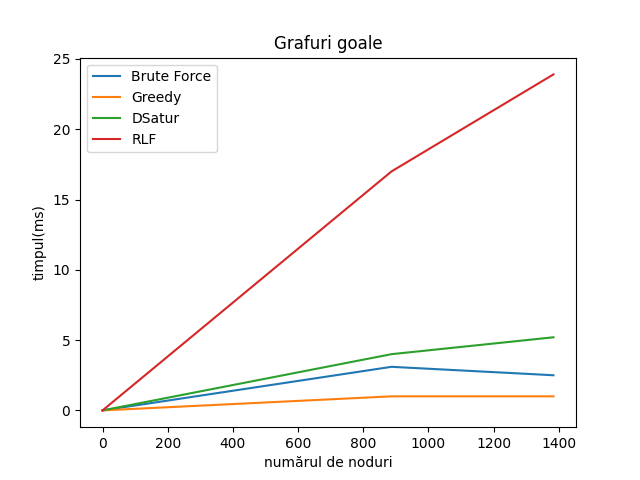
\includegraphics[width=\textwidth]{fig1.eps}
% \caption{A figure caption is always placed below the illustration.
% Please note that short captions are centered, while long ones are
% justified by the macro package automatically.} \label{fig1}
% \end{figure}

% ------------------------------------------------------------------------------

%
% ---- Bibliography ----
%
% BibTeX users should specify bibliography style 'splncs04'.
% References will then be sorted and formatted in the correct style.
%
% \bibliographystyle{splncs04}
% \bibliography{mybibliography}
%
\begin{thebibliography}{8}

\bibitem{1}
J. Bondy and U. Murty, Graph Theory - Graduate Texts in Mathematic.
Springer, 2008.
\bibitem{2}
Z. \`{A}d\`{a}m Mann and A. Szajk\`{o}, “Average-case complexity of backtrack
search for coloring sparse random graphs,” Journal of Computer and
System Sciences, vol. 79, no. 8, pp. 1287–1301, 2013.
\bibitem{3}
“Backtrack: An o(1) expected time algorithm for the graph coloring
problem,” Information Processing Letters, vol. 18, no. 3, pp. 119–121,
1984.
\bibitem{4}
N. Barnier and P. Brisset, “Graph coloring for air traffic flow management,” 
Annals of Operations Research, vol. 130, 03 2002.
\bibitem{5}
“The application of a graph coloring method to an examination scheduling problem,” 
Institute for Operations Research and the Management
Sciences (INFORMS), vol. 11, no. 5.
\bibitem{6}
A. Murat and B. Nurdan, “A performance comparison of graph coloring algorithms,” 
International Conference on Advanced Technology
Sciences (ICAT’16), vol. 4, pp. 1–19, 12 2016
\bibitem{7}
Z. Mann, “Complexity of coloring random graphs: An experimental
study of the hardest region,” Journal of Experimental Algorithmics,
vol. 23, pp. 1–19, 03 2018
\bibitem{8}
\href{https://acs-aa-challenge.github.io/acs-aa-challenge/18-np-2-colouring/}{Enunțul problemei}
\bibitem{9}
M. Garey and D. Johnson, Computer and Intractability: A Guide to the
Theory of NP-Completeness, 01 1979.
\bibitem{10}
D. Porumbel, J.-K. Hao, and P. Kuntz, “An evolutionary approach with
diversity guarantee and well-informed grouping recombination for graph
coloring,” Computers Operations Research, vol. 37, pp. 1822–1832, 10
2010.
\bibitem{11}
L. Ouerfelli and H. Bouziri, “Greedy algorithms for dynamic graph coloring,” 2011 International Conference on Communications, Computing
and Control Applications, CCCA 2011, 03 2011.
\bibitem{12}
\`{A}. E. Eiben, J. K. Van Der Hauw, and J. I. van Hemert, “Graph coloring
with adaptive evolutionary algorithms,” Journal of Heuristics, vol. 4,
no. 1, pp. 25–46, 1998.
\bibitem{13}
D. Br\`{e}laz, “New methods to color the vertices of a graph,”  Commun.
ACM, vol. 22, pp. 251–256, 04 1979.
\bibitem{}
\href{https://en.wikipedia.org/wiki/Graph_coloring}{Graph coloring - Wikipedia}
\bibitem{}
\href{https://citeseerx.ist.psu.edu/document?repid=rep1&type=pdf&doi=203a7b17267a28a06808bfb3b0b9571e32d15503}{A Comparison of Parallel Graph Coloring Algorithms}
\bibitem{}
\href{https://dergipark.org.tr/en/download/article-file/254140}{A Performance Comparison of Graph Coloring Algorithms}
% \bibitem{}
% \href{https://github.com/brrcrites/graph-coloring}{Graph coloring C++ library}
\bibitem{}
\href{https://curs.upb.ro/2022/mod/folder/view.php?id=77105}{Moodle - Analiza algoritmilor}
% 
\end{thebibliography}
\end{document}
